\chapter{ICESym y MRCVC}

El Simulador de Motores de Combustión Interna (ICESym) permite la simulacion de
motores tanto alternativos como rotativos en general y el MRCVC en particular.
%
En su código se incluyen modelos de la geometría del motor, la transferencia
de calor y el solape de cámaras.

\section{Simulación computacional del ciclo termodinámico MRCVC}

% \section{ICESym}
Para simular el ciclo operativo del motor, se utilizó el simulador de motores
de combustión interna ICESym \cite{icesym}, desarrollado en conjunto por la
UNCo y UNL.
%
Este simulador utiliza modelos unidimensionales para simular el flujo en los
conductos de admisión y escape y modelos cero dimensionales o termodinámicos
para la cámara de combustión, la transferencia de calor y los modelos de
fricción.
%

Incluye un modelo para el solape entre cámaras \cite{lopez16} y modificaciones
particulares al MRCVC, para este trabajo en particular  y con el fin de obtener
una mapa del coeficiente de descarga, se ha agregando la diferencia de presión
entre cámara y puerto como variable de modo que $Cd = f(L_v, \delta P)$.
%
En trabajos anteriores se tienen estudios más detallados del MRCVC, por lo que
aquí se presenta de manera breve los aspectos geométricos y mecánicos del motor
que son relevantes a este trabajo.

\subsection{Geometría}
%
La geometría del MRCVC permite que gran parte de la combustión se de a volumen
constante\cite{mrcvc_geom}, por lo que se espera un rendimeinto mayor en
comparación al ciclo otto de un motor convencional de encendido por chispa.
%
Para un MRCVC con $n$ paletas de radio nulo la geometría como función del
ángulo del cigüeñal queda totalmente definida por el radio de trayectoria de
paletas $R$, semiancho de paletas $r$ y altura de cámara $h$.

\subsection{Ciclo operativo}
% La combustión se realiza a volumen constante, por lo que es de esperarse
% mayores rendimientos de conversión de combustible en relación a motores en los
% que la combustión no se realiza a volumen constante.

% hace falta mostrar que esto es así? poner algún gráfico del heywood o cosas
% por el estilo. puedo citar el heywood?

En otros trabajos se detallo el ciclo operativo del motor, la variación de la
geometría y el funcionamiento en detalle de ICESym, así como también el modelo
de solape de cámaras desarrollado para el uso con el MRCVC.
%

Para una misma relación de compresión, una combustión a volumen constante
alcanza valores de presión y temperatura mayores en comparación a otros ciclos.
%
Este presenta un mayor rendimiento térmico
\begin{figure}
    \centering
    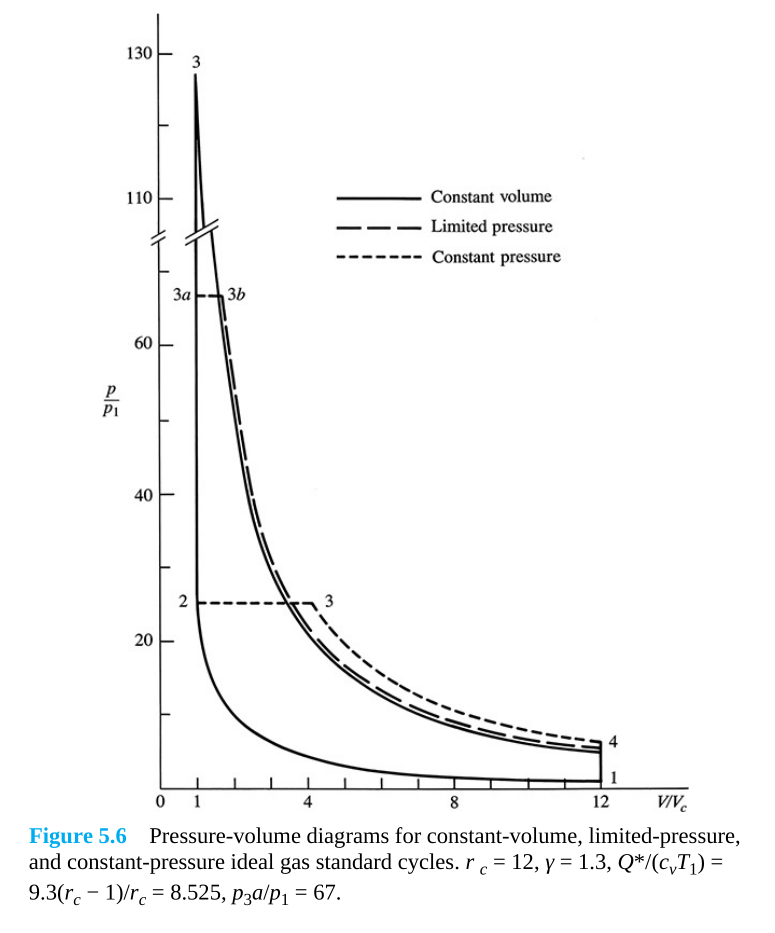
\includegraphics[width=1\textwidth]{comparacion_ciclos.png}
    \caption{Comparación de ciclos ideales (cambiar por una imagen propia}
    \label{fig:comparacion_ciclos}
\end{figure}

En la figura \ref{fig:comparacion_rendimientos} se ve como para una $r_c$ dada,
el ciclo a volumen constante tiene el mayor rendimiento.

\begin{figure}
    \centering
    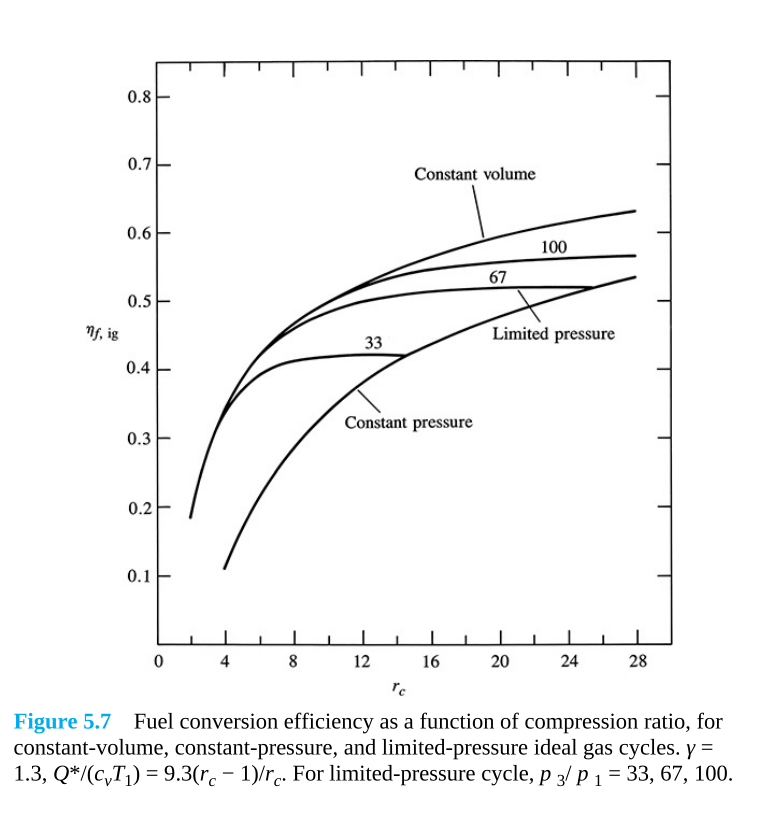
\includegraphics[width=1\textwidth]{rendimiento_conv_comb.png}
    \caption{Comparación de rendimientos (cambiar por una imagen propia}
    \label{fig:comparacion_rendimientos}
\end{figure}


% La combustión se realiza casi en su totalidad a volumen constante
%
% El gas de admisión es una mezcla estequeométrica de aire y vapor de combustible
% perfectamentes mezclados.
%
% En caso de que exista flujo revertido, este no se mezcla con el gas fresco,
% sino que se vuelve a admitir.
%
% No se tienen en cuenta las péridas de masa por los huelgos entre partes
% móviles(\emph{crevice flow})
%
% La combustión se simula con el modelo de liberación de calor de Weibe

El indicador que se tomará como referencia para evaluar y comparar diferentes
geometrías es el rendimiento volumétrico ($\eta_v$), este parámetro se define
como:

\begin{equation}
    \eta_v = \frac{m_a}{\rho_{a,i}V_d}
\end{equation}

Dónde:
%
\begin{description}
    %
    \item[$m_i$] es la masa de mezcla fresca inductada
        %
    \item[$\rho_{a,i}$] es la densidad del aire en el puerto de admisión
        %
    \item[$V_d$] es el volumen desplazado
        %
\end{description}

El rendimiento volumétrico tiene una dependencia compleja de varios factores,
este parámetro es el que da forma a las curvas de \emph{performance} que se
suelen ver en literatura ya que indica la cantidad de mezcla fresca disponible
para la combustión. 
%
En en caso de motores de inyección directa (tanto de CI SI)

\section{Sistemas de intercambio de gases}
%
\subsection{Área de referencia}
%
El área de referencia utilizada por ICESym es el área de cortina.

$$ A_R = A_C = \pi D_v L_v $$

\subsection{Solape de cámaras}
%
Tanto al inicio como al cierre del puerto se ve solape de cámaras, por lo que
en estos intervalos angulares hay un valor de $C_D$ para cada cámara.

\section{CAD}
%
El modelo 3D de los puertos de admisión, escape y los componentes internos del
motor que afectan el flujo y son relevantes a la flujometría se realizaron con
FreeCAD\cite{freecad} para generar un archivo en formato $.BREP$ y luego
salome\cite{salome} para obtener un archivo .stl "cerrado" en formato ASCII

Dada la cantidad de geometrías posibles y el tiempo que toma el proceso, se
realizaron algunas simplificaciones

\section{Geometría}
%
El puerto se hace recto, igual se podría hacer una entrada más suave.

La altura de la ranura se adopta en 2/3 del alto de la cámara, siendo $h_c=0.0441\ mm$

El eje del puerto se hace perpendicular a una línea que pasa entre el centro
del motor y el la línea media del puerto.

% En este capítulo describo como es el procedimiento realizado en cada paso de
% la optimización:

% -> optimización algoritmo genético y simulación con icesym, tendría que
%    explicar como funciona icesym y el optimizador
% -> freecad + salome
% -> openfoam
\section{Metodología}
%
Se simulará un MRCVC de 3 paletas usando el simulador de motores de combustión
interna ICESym \cite{icesym} con el propósito de obtener curvas de rendimiento
volumétrico.
%
Estas serán el principal criterio para evaluar el diseño de los sistemas de
intercambio de gases, que consisten de los puertos y conductos de admisión y
escape.
%
La geometría se optimizará mediante un algoritmo genético, el cual transforma
los datos de rendimiento volumétrico en un puntaje representativo de cada
motor.


La simulación con ICESym requiere del conocimiento previo de los coeficientes
de descarga de los puertos los cuales inicialmente serán estimados para poder
realizar la primer iteración con el simulador.
%
Se utilizará la geometría obtenida en esta primer iteración para crear modelos
en CAD de los puertos de admisión y escape para realizar flujometrías virtuales
y así poder obtener los coeficientes de descarga de cada puerto en distintos
grados de apertura.


\section{Modificaciones a ICESym} \subsection{Coeficiente de descarga}
%
Se introdujo una opción para poder ejecutar ejectura ICESym con un modelo de
$C_d$ que dependa de dos variables, diferencia de presión y \emph{alzada}.
%
Esto significó agregar una opcion que permita seleccionar entre un Cd que
depende únicamente de la alzada o de una o dos variables.

Con esto se construye una mapa del coeficiente de descarga de la forma $C_d =
f(lv, dp)$, que se utiliza en \emph{def\_valve.f90} para calcular el área
efectiva de la válvula.
%
En la porción de código que sigue, se llama la rutina interpolant para calcular
el valor de Cd para un valor de Lv dado, en caso de utilizar el modelo de dos
variables, se llama la rutina interpolant2d.
%
Ambas realizan una interpolación lineal entre los valores conocidos de Cd.


\begin{lstlisting}[language=fortran]
SUBROUTINE area_valve(theta, Dv, VO, VC, Lvmax, Nval, type_dat, &
    Lv_array, cd_model, Cd, Cd_lv, Cd_dp, deltaP, theta_cycle, F_v)
    [...]
     IF (cd_model .EQ. 0) THEN
        CALL interpolant(Cd(:, 1), Cd(:, 2), Lv, Cd_int)
     ELSE
        CALL interpolant2d(Cd_lv, Cd_dp, Cd, Lv, deltaP, Cd_int)
     END IF
     F_v = Cd_int*Nval*pi*Dv*Lv
    [...]
END SUBROUTINE area_valve
\end{lstlisting}


\section{Notas}
Algunas notas sobre el mrcvc o la simulacion de icesym que todavia no tienen
lugar.

\begin{enumerate}
    \item La temperatura de pared se asume en 450 K
    \item El área de referencia es el área de cortina
    \item No cambie la cantidad de puntos en que se discretiza cada tubo
    \item Agregue una interpolación 2D para el cálculo del Cd
    \item La combustión es estequeométrica con $a_weibe=5$ y $m_weibe=2$
    \item El modelo de combustión es 1
    \item scavange = 0
    \item El combustible utilizado es \emph{isooctano} y tiene estas
        caracteristicas 
        \begin{itemize}
            \item $y = 2.25$
            \item $H_{vap} = 2.25 MJ/kg$
            \item $Q_{fuel} = 44 MJ/kg_f$
        \end{itemize}
\end{enumerate}

\section{Dudas}
Con respecto al diccionario de configuración de ICESym:

\begin{enumerate}
    \item ¿Que es histo?
    \item ¿Que es position?
\end{enumerate}

